\section{ViQ: Visual Quantized Representations}
\label{sec:method}

The visual quantization training for ViQ follows a two-stage process, as depicted in Fig.~\ref{fig:approach}. In Stage 1, text-aligned pre-training is performed on continuous features to enhance multimodal alignment. Subsequently, Stage 2 applies quantization in a progressive manner.

\subsection{Text-Aligned Pre-Training at Any Resolution}
\label{sec:methods_1}

The first stage of ViQ training aims to create a visual encoder that functions in a multi-modal manner. This is accomplished by leveraging text-aligned visual pre-training to align the vision and language embeddings within ViQ, thereby following an optimization strategy similar to conventional multi-modal training.

\paragrapha{Any Resolution Adaptation. }While Language-Image Pre-training models such as CLIP~\cite{radford2021clip} and SigLIP~\cite{zhai2023siglip} offer a strong initialization for building multi-modal visual encoders, most existing models are constrained by a fixed input size. In multi-modal learning, native image resolution often provides a more natural and efficient form of visual representation. To overcome the limitations of fixed-scale pre-training, we follow the approach of NaViT~\cite{dehghani2024navit} and replace the original positional embedding layer with one that supports an adequately dimensioned size. This allows the model to resize positional parameters when processing images at arbitrary resolutions dynamically. We adopt the techniques introduced in OryxViT~\cite{liu2024oryx} to maintain computational efficiency with variable-length visual tokens.

\begin{figure*}[t]
\centering
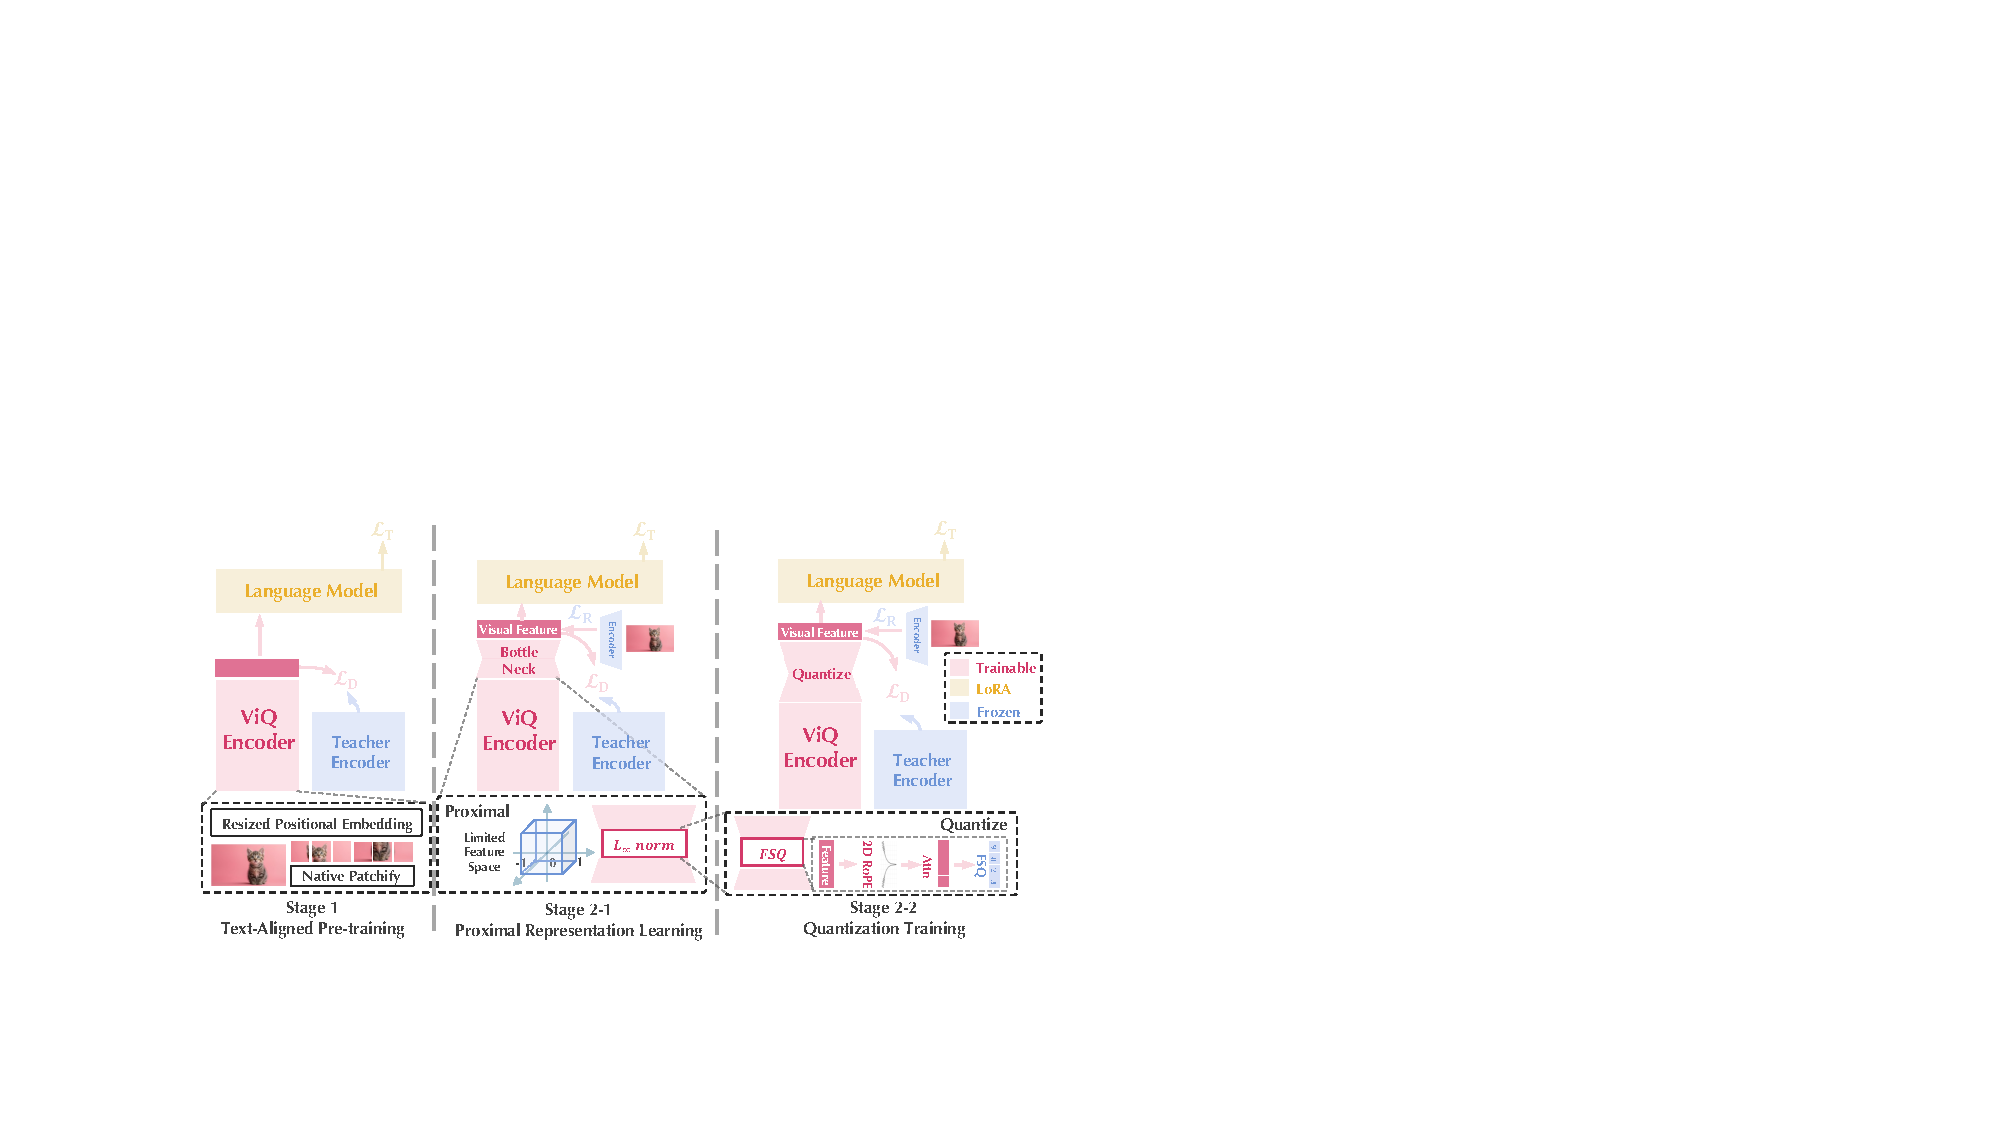
\includegraphics[width=\linewidth]{figures/fig2_eccv.pdf}
\caption{\textbf{Approach of ViQ Representation Learning.} Stage 1 enables multimodal alignment with language supervision, while Stage 2 compresses the high-dimensional visual features into discrete codes in a progressive learning manner. }
\label{fig:approach}
\end{figure*}

\paragrapha{Text-Guided Multi-Modal Pre-training. }We optimize the continuous feature space of ViQ to be more compatible with multi-modal learning during our text-aligned pre-training stage. Specifically, given a data triplet $[I, T, A]$ consisting of an image $I$, a text query $T$, and an answer $A$, we employ a temporary language model to compute the text supervision loss $\mathcal{L}_{\text{text}}$, which is defined as:
\begin{equation}
    \mathcal{L}_{\text{text}}=\text{Cross Entropy}[\ \text{LLM}(\text{ViQ}(I),\ T),\ A]
\end{equation}

\paragrapha{Self Distillation. }During the multi-modal pre-training stage, we apply self-distillation to regularize the ViQ model, preventing it from overfitting to the multi-modal data and disregarding the knowledge acquired from large-scale language-image pre-training, which is crucial for maintaining the generalizability and foundational capabilities. We use the original fixed-resolution model as the teacher to supervise the cosine similarity of the semantic token (i.e., the class token in mainstream architectures), ensuring that the representations produced at any resolution preserve the original high-level semantic information:
\begin{equation}
    \mathcal{L}_{\text{distill}} = 1 - \cos\left(\mathbf{z}_s^{\text{student}}, \mathbf{z}_s^{\text{teacher}}\right)
\end{equation}
where \(\mathbf{z}_s^{\text{student}}\) and \(\mathbf{z}_s^{\text{teacher}}\) denote the semantic tokens from the student (any-resolution) and teacher (fixed-resolution) models, respectively.

\paragrapha{Training Recipe for Native Resolution. }We employ a progressive training strategy that transitions from fixed-resolution to any-resolution inputs. Specifically, the training begins with low-resolution images at their native aspect ratios, and the total number of pixels is gradually increased throughout the training process until native resolution is attained. During training, multi-modal data are packed to fit the maximum token length for higher pre-training efficiency. The image complexity, question-answering difficulty, and overall sequence length are progressively raised to steadily adapt the model to multi-modal tasks. Further implementation details are provided in the appendix. We combine the text loss \(\mathcal{L}_{\text{text}}\) and the distillation loss \(\mathcal{L}_{\text{distill}}\) for joint optimization.

\subsection{Visual Quantized Representation Learning}
\label{sec:methods_2}

The second stage of ViQ training involves quantizing the continuous features into discrete codes. A core challenge in this process is to fully optimize the discrete representation space so as to preserve fine-grained visual information. Through our approach, we demonstrate that the resulting ViQ representations are effective in supporting high-quality visual understanding in multimodal contexts.

\paragrapha{Proximal Representation. }The primary objective of quantization is to map continuous visual features from a high-dimensional space $\mathbb{R}^{C}$ into a constrained discrete space defined by a codebook $\mathcal{Z}$. However, we observe that directly quantizing high-dimensional visual features results in significant precision loss. To mitigate this, our proposed ViQ method progressively reduces the complexity of the latent space using a proximal representation. Given a high-dimensional visual feature $f \in \mathbb{R}^C$, we first apply a bottleneck layer to compress it into an intermediate-dimensional feature $f_1 \in \mathbb{R}^D$. We then further constrain the feature space complexity via a regularization function, referred to as a proximal representation. In our implementation, we apply the $L_\infty$-norm to the compressed latent feature, projecting all features onto a hypercube surface such that $\lVert f_1 \rVert_\infty = 1$. This step progressively reduces the feature space complexity prior to discrete quantization. The proximal representation helps regulate the distance between features and quantization anchors, thereby reducing information loss during quantization. The bottleneck compression operations can be formulated as:
\begin{equation}
\begin{aligned}
    f_1=L_{\infty}(\text{BN}(f)), \hat{f}=\text{BN}'(f_1)
\end{aligned}
\end{equation}
where $\text{BN}$ denotes the bottleneck fully connected layer for dimension compression and $\text{BN}'$ denotes the inverted bottleneck layer respectively.

\paragrapha{Multi-Head Finite Scalar Quantization. }After learning an initial continuous proximal representation within a constrained latent space, we replace the normalization function with a bottleneck downsampling layer that projects the latent features into a lower-dimensional space \( f_2 \in \mathbb{R}^d \), where \( d \ll D \ll C \). The final dimension \( d \) is kept sufficiently small to facilitate effective quantization. We employ Finite Scalar Quantization (FSQ)~\cite{mentzerfinite} to discretize the compact continuous features \( f_2 \), as this method offers stable training behavior without requiring additional optimization during quantization. The FSQ process can be formulated as:
\begin{equation}
z = \text{round}(\mathcal{Q}(f_2))
\end{equation}
where $\mathcal{Q}$ indicates the Finite Scalar Quantization function.

To enhance the representational capacity of the quantized codes, we utilize a multi-head attention mechanism that expands each visual patch into \( 2 \times 2 \) visual codes. Specifically, the latent feature \( f_2 \in \mathbb{R}^{B \times N \times d} \) is up-projected to \( \mathbb{R}^{B \times 4N \times d} \), where \( N \) denotes the number of original image patches. The expanded patches are then processed via multi-head self-attention across each patch. After self-attention, the tokens are concatenated along the token dimension prior to quantization. Following quantization, the sequence length is restored via a projection layer to maintain the original visual downsampling rate. It is important to note that the expanded image patches are processed independently; as a result, the quantized representations in ViQ remain independent, making them more suitable for representation learning and downstream tasks.

\paragrapha{Rotary Position Embedding. }For quantized representations at arbitrary resolutions, we incorporate a 2D rotary position embedding (RoPE)~\cite{su2024roformer} to explicitly encode spatial resolution information. The RoPE layer is inserted prior to the quantization step. Specifically, 2D RoPE extends the 1D RoPE formulation used in large language models by embedding both height and width information of the visual content. Given a token feature \( f_m \in \mathbb{R}^d \) at position \( (h, w) \) in the 2D feature map, the rotary encoding is applied as:
\begin{equation}
\tilde{f}_m = f_m \odot e^{i (h \theta_h + w \theta_w)}
\end{equation}
where \( \theta_h \) and \( \theta_w \) are frequency parameters for the height and width dimensions, respectively, and \( \odot \) denotes element-wise multiplication with complex exponentials. This formulation ensures that relative spatial relationships are preserved across varying resolutions.

\begin{table*}[t]
  \centering
  \caption{\textbf{Comparison results on multi-modal understanding tasks.} We conduct experiments with various visual encoder counterparts on general multi-modal benchmarks. All the methods are trained with the same data collection.}
  \begin{adjustbox}{width=\linewidth}
    \begin{tabular}{lccccccccccccc}
    \toprule
    \multicolumn{4}{c}{Base LLM}        & \multicolumn{1}{c}{\multirow{2}[4]{*}{\rotatebox{30}{MMStar}}} & \multicolumn{1}{c}{\multirow{2}[4]{*}{\rotatebox{30}{MMMU}}} & \multicolumn{1}{c}{\multirow{2}[4]{*}{\rotatebox{30}{SimpleVQA}}} & \multicolumn{1}{c}{\multirow{2}[4]{*}{\rotatebox{30}{InfoVQA}}} & \multicolumn{1}{c}{\multirow{2}[4]{*}{\rotatebox{30}{TextVQA}}} & \multicolumn{1}{c}{\multirow{2}[4]{*}{\rotatebox{30}{DocVQA}}} & \multicolumn{1}{c}{\multirow{2}[4]{*}{\rotatebox{30}{OCRBench}}} & \multicolumn{1}{c}{\multirow{2}[4]{*}{\rotatebox{30}{AI2D}}} & \multicolumn{1}{c}{\multirow{2}[4]{*}{\rotatebox{30}{ChartQA}}} & \multicolumn{1}{c}{\multirow{2}[4]{*}{\rotatebox{30}{Avg.}}} \\
\cmidrule{1-4}    \multicolumn{1}{c}{Visual Encoder} & Size  & AnyRes & Discrete &       &       &       &       &       &       &       &       &       &       \\
    \midrule
    \multicolumn{4}{c}{\textit{Qwen2.5 - 1.5B}} \\
    \midrule
    OAI-CLIP-L~\cite{radford2021clip} &   0.3B    & \ding{55}  &   \ding{55}   &44.9 &	40.7 	&21.3 &	24.2 	&58.9 &	52.9 &	460.0 &	68.1 	&55.0 &	45.8 \\
    SigLIP2-g~\cite{tschannen2025siglip} & 1.1B    & \ding{55}   &\ding{55}  &48.1 	 &42.4  &	25.6  &	28.2 	 &73.1  &	67.8  &	590.0  &	71.5  &	62.0 	 &53.1  \\
    DinoV2-g~\cite{oquab2023dinov2} &   1.1B    & \ding{55}     &   \ding{55}     &     47.1 	&41.8 	&24.0 	&31.7 	&72.1 &	76.9 	&619.0 	&68.8 	&61.8 	&54.0 \\
    \midrule
    OryxViT~\cite{liu2024oryx}  & 0.4B  &  \ding{51}      &   \ding{55}     &    46.4   &  42.1     &   23.2    &   31.8    &   71.8    &   73.5    &   622.0    &    68.2   &    62.1   &   53.4  \\
    AIMv2-H~\cite{fini2025multimodal} &   0.7B    & \ding{55}    &   \ding{55}     & 48.5 &	41.8 &	23.5 	&31.9 	&71.6 	&73.7 &	623.0 &	69.8 &	62.5 &	53.9   \\
    InternViT-2.5~\cite{chen2412expanding} & 0.3B  & \ding{55}     &   \ding{55}     & 47.9&  	40.3 	& 23.6 	& 35.5 & 	73.0 & 	81.7 & 	681.0 & 	69.6 & 	\textbf{69.2} & 	56.5  \\
    InternViT-2.5-6B~\cite{chen2412expanding} & 6.0B & \ding{55}     &   \ding{55}     & \textbf{48.5}&  	42.1 & 	23.7 	& 35.2 & 	\textbf{75.5} & 	80.1 & \textbf{690.0} & 	\textbf{70.7} & 	67.8 & 	57.0  \\
    \midrule
    QLIP~\cite{zhao2025qlip}  &   0.3B    & \ding{55}    &    \ding{51}  &39.9 &	36.9 &	13.7 &	14.8 &	45.1 &	12.2 &	290.0 &	61.9 	&14.1 &	29.7 \\
    UniTok~\cite{ma2025unitok} &   0.3B    &  \ding{55}      &   \ding{51}  &  41.0 &	36.1 &	15.5 	&15.9 &	39.7 &	11.6 	&323.0 &	61.2 &	43.8 &33.0  \\
    \midrule
    \rowcolor{red!10} ViQ & 1.3B  &   \ding{51}     &   \ding{51}     & 47.8  & \textbf{42.6}  & \textbf{26.0}  & \textbf{41.6}  & 74.3  & \textbf{84.2}  & 636.0  & 69.7  & 65.2  & \textbf{57.2}\\
    \midrule
    \multicolumn{4}{c}{\textit{Qwen2.5 - 7B}} \\
    \midrule
    OAI-CLIP-L~\cite{radford2021clip} &    0.3B   &  \ding{55}      &     \ding{55}   & 53.9 & 	47.1 & 	25.4 & 	33.9 	& 66.4 	& 61.4 & 	544.0 & 	76.6 & 	65.1 	& 53.8 \\
    SigLIP2-g~\cite{tschannen2025siglip} & 1.1B    & \ding{55}    &   \ding{55}     & \textbf{57.2} &	48.3 &	28.5 &	37.3 &	78.7 &	75.0 	&671.0 &	\textbf{79.5} &	72.8 &	60.5   \\
    \midrule
    OryxViT~\cite{liu2024oryx} & 0.4B &  \ding{51}      &  \ding{55}      &   56.4    &    48.1   &   26.5    &   39.9    &   78.5   &  79.8  &    660.0   &  78.2     &   72.1      & 60.6  \\
    AIMv2-H~\cite{fini2025multimodal} &    0.7B    & \ding{55}     &   \ding{55}     & 55.2 &	48.2 &	26.8 &	41.8 &	79.1 &	80.1 	&687.0 	&77.8 &	72.5 &	61.1 \\
    InternViT-2.5-6B~\cite{chen2412expanding} &   6.0B     & \ding{55}     &  \ding{55}      & 55.3 &	48.1 &	28.4 &	44.9 &	\textbf{79.9} &	85.7 &	\textbf{757.0} &	78.7 &	\textbf{77.4} 	&63.8 \\
    \midrule
    \rowcolor{red!10} ViQ & 1.3B  &   \ding{51}    &   \ding{51}     & 54.2  & \textbf{49.1}  & \textbf{28.5}  & \textbf{55.3}  & 78.5  & \textbf{88.9}  & 711.0   & 76.7  & 72.8  & \textbf{63.9}  \\
    \bottomrule
    \end{tabular}
  \end{adjustbox}
  \label{tab:multimodal}
\end{table*}

\paragrapha{Multi-Stage Training with Low-Level Supervision. }Building upon the progressive quantization framework, we learn the compressed feature representation in a multi-stage manner. First, starting from the proximal representation in the constrained space, we introduce a bottleneck layer with a regularization function between the continuous input features and the final output. We retain both the text loss \(\mathcal{L}_{\text{text}}\) and the self-distillation loss \(\mathcal{L}_{\text{distill}}\) during this phase, keeping all other settings consistent with Stage 1 training. To enhance low-level detail preservation and improve latent feature quality, we incorporate a pre-trained visual autoencoder that encodes the original input images into the low-level latent features. This encoding is supervised using a VAE-style latent loss along with a negative log-likelihood (NLL) term, expressed as:
\begin{equation}
\mathcal{L}_{\text{recon}} = \text{NLL}(\hat{f}, \text{Encoder}(x))
\end{equation}
where \(x\) denotes the input image and $\hat{f}$ denotes the recovered features after compression or quantization. Here the NLL term is computed under a Gaussian likelihood with fixed (unit) variance over the target VAE latent $\text{Encoder}(x)$, so that the loss reduces, up to a constant, to a mean-squared error between $\hat{f}$ and $\text{Encoder}(x)$, i.e., $\mathcal{L}_{\text{recon}} = \tfrac{1}{2}\lVert \hat{f} - \text{Encoder}(x)\rVert_2^2 + \text{const}$. This makes the objective a simple and stable regression on the pre-trained VAE latent space rather than a pixel-level reconstruction.

Once the bottleneck compression is adequately learned, we replace the proximal regularization function with a quantization module in the subsequent quantization training stage. Since our vector quantization (VQ) implementation is optimization-free, no additional codebook supervision is required at this stage. The overall training objective combines the three losses as follows:
\begin{equation}
\mathcal{L}_{\text{total}} = \lambda_{\text{text}}\mathcal{L}_{\text{text}} + \lambda_{\text{distill}}\mathcal{L}_{\text{distill}} + \lambda_{\text{recon}}\mathcal{L}_{\text{recon}}
\end{equation}
